\documentclass[11pt]{article}

\usepackage[english]{babel}
\usepackage[utf8]{inputenc}
\usepackage{graphicx}
\usepackage{amsmath,amssymb}
\usepackage{subcaption}
\usepackage{hyperref, url}
 \usepackage[table,xcdraw]{xcolor}
 \usepackage[font=small,labelfont=bf]{caption}
\parindent 0mm
\parskip 1mm

% add your name and student number in parenthesis
\title{Survival Analysis of TCGA Liver cancer expressed gene transcript }
\author{ Sailendra Pradhananga (sailendra.pradhanaga@scilifelab.se)\\ \\
			Project Report:Algorithms in Bioinformatics}

\begin{document}

\maketitle

\section{Introduction}


Survival analysis are statistical toolkits that are used to analyzing the outcome of variables based on time period of event occurrence. The event could be either be death, outbreak of disease or failure of automobile parts which are then followed specified time period in days, weeks or years. The major part of the these type of data involves two kinds of variables: first is the time to event and second whether the event have occurred or not. Based on different methods such as non parametric model such Kaplan Meier method or regression model such as cox proportional hazards two function, survival function and hazard function. The survival function gives the probability  for each time-points of surviving up to that events while hazard function whether the event has occurred or not  given the individual has survived or not. The main aim of these type of analysis is find the relationship between the survival time and variables under study such as drugs, gene expression, treatment  either with different covariates such as age, gender, race.

In the current project, we are provided a liver cancer patients of different races  dataset survival time and gene expression dataset of various grades. The main aim was to model the data with survival model in order find the potential prognostic marker for survival of patients using Cox Proportional Hazard models. Additionally, using the multiple hypothesis correction we predicted 4698 gene transcripts at 0.05 FDR. 

\section{Method}

	\subsection{TCGA Dataset}
The  TCGA dataset for the analysis was download from the (http://kaell.org/files/survivalLIHC.txt) site. As already stated in the project guidelines, these are the cancer patient expression data from the sequenced liver tumor.  Additionally there are few other features implication each cancer patient ethnicity, sex and cancer types.  These data were first read into python notebook as pandas data frame  as done in  jupyter notebook.  Additional exploratory analysis was done in the notebook itself. The  dataset consists of both categorical features and numerical data of gene expression dataset. 

	\subsection {Preprocessing of Dataset}
In the survival analysis, the different categorical features were provided of liver cancer patients. These categorical features includes Gender, Race, Stage , Status, Age and LivingDays of different cancer patients.  These categorical features were then coded into different numerical codes . Originally, the dataset consists of gene expression profile os $19,571$. Furthermore, only those gene expression data were taken which had at least an expression in one of the patients.  

	\subsection{Cox proportional Hazard model}
	 Cox proportional hazards regression, used to relate several risk factors or exposures, considered simultaneously, to survival time. In the current project we used the implementation of Cox regression hazard model implemented on lifelines packages. Although I had tried including other covariates such as age and temperature to be used in the model, at this phase we have used individual expression of each gene transcript iteratively in order to get hazard function and survival rates of each gene transcripts. Based on proportional hazard model we get an p-value estimates of gene transcript. However not all the gene transcripts fitted into the Cox survival model thus we excluded to get final list of pvalues for each transcripts. implementation in lifelines \cite{lifelines} 
	 
	\subsection {Multiple testing correction}
	As discussed in earlier exercises we have  implemented multiple testing correction for all the p.value estimates of gene expression for liver cancer to occur. However since we are testing multiple features, the pvalue $<$ 0.05 might be too lenient estimates. Hence based on storey and tribasni papser \cite {} an q value estimates were made of all the pvalues calculated. We fitted the cubic spline in the $\pi_0$ estimates in the given  $\lambda$ values.
	 


 \section{Result}
 
 	
	
	\subsection {TCGA Liver Cancer cohort characterstics}
 
The cancer cohort consists of different phenotypic features such liver cancer types, age, gender, which are further summarized in table~\ref{tab:table1} . Importantly, the important dependent variable is the status of an patient cohort  and the  living days which is the measure of the time of survival.. The average living days for alive  patient cohort is  896.80 while for dead sample cohort is 655.21 with pvalues $< 0.001$ as figure~\ref{fig:status_livingdays}
 
 \begin{table}[h]
\centering
\scalebox{0.5}{
	\begin{tabular}{|l|l|}
	\hline
		\multicolumn{2}{|l|}{\cellcolor[HTML]{96FFFB}{\color[HTML]{FE0000} Summary statistics of TCGA liver cancer cohorts}}                                                                                                                                 	\\ \hline
		\multicolumn{2}{|c|}{Gender}                                                                                                                                                                                                                         	\\ \hline
			\begin{tabular}[c]{@{}l@{}}male\\ \\ female\end{tabular}                                                                                                       & \begin{tabular}[c]{@{}l@{}}245\\ \\ 		119\end{tabular}                               \\ \hline
		\multicolumn{2}{|c|}{Race}                                                                                                                                                                                                                           \\ \hline
			\begin{tabular}[c]{@{}l@{}}white\\ asian\\ black or african american\\ not reported\\ american indian or alaska native\end{tabular}                             & \begin{tabular}[c]{@{}l@{}}182\\ 154\\ 17\\ 10\\ 1\end{tabular}                    \\ \hline
		\multicolumn{2}{|c|}{Liver cancer stage}                                                                                                                                                                                                             \\ \hline
			\begin{tabular}[c]{@{}l@{}}stage i\\ stage ii\\ stage iiia\\ not reported\\ stage iiic\\ stage iiib\\ stage iii\\ stage ivb\\ stage iv\\ stage iva\end{tabular} & \begin{tabular}[c]{@{}l@{}}170\\ 83\\ 63\\ 24\\ 9\\ 8\\ 3\\ 2\\ 1\\ 1\end{tabular} \\ \hline
		\multicolumn{2}{|c|}{Status}                                                                                                                                                                                                                         \\ \hline
		\begin{tabular}[c]{@{}l@{}}alive\\ dead\end{tabular}                                                                                                            & \begin{tabular}[c]{@{}l@{}}234\\ 130\end{tabular}                                  \\ \hline
	\end{tabular}}
\caption{Summary Statistics of TCGA liver cancer cohort \tiny}
\label{tab:table1}
\end{table}

\begin{figure}[tbh]
    \centering
      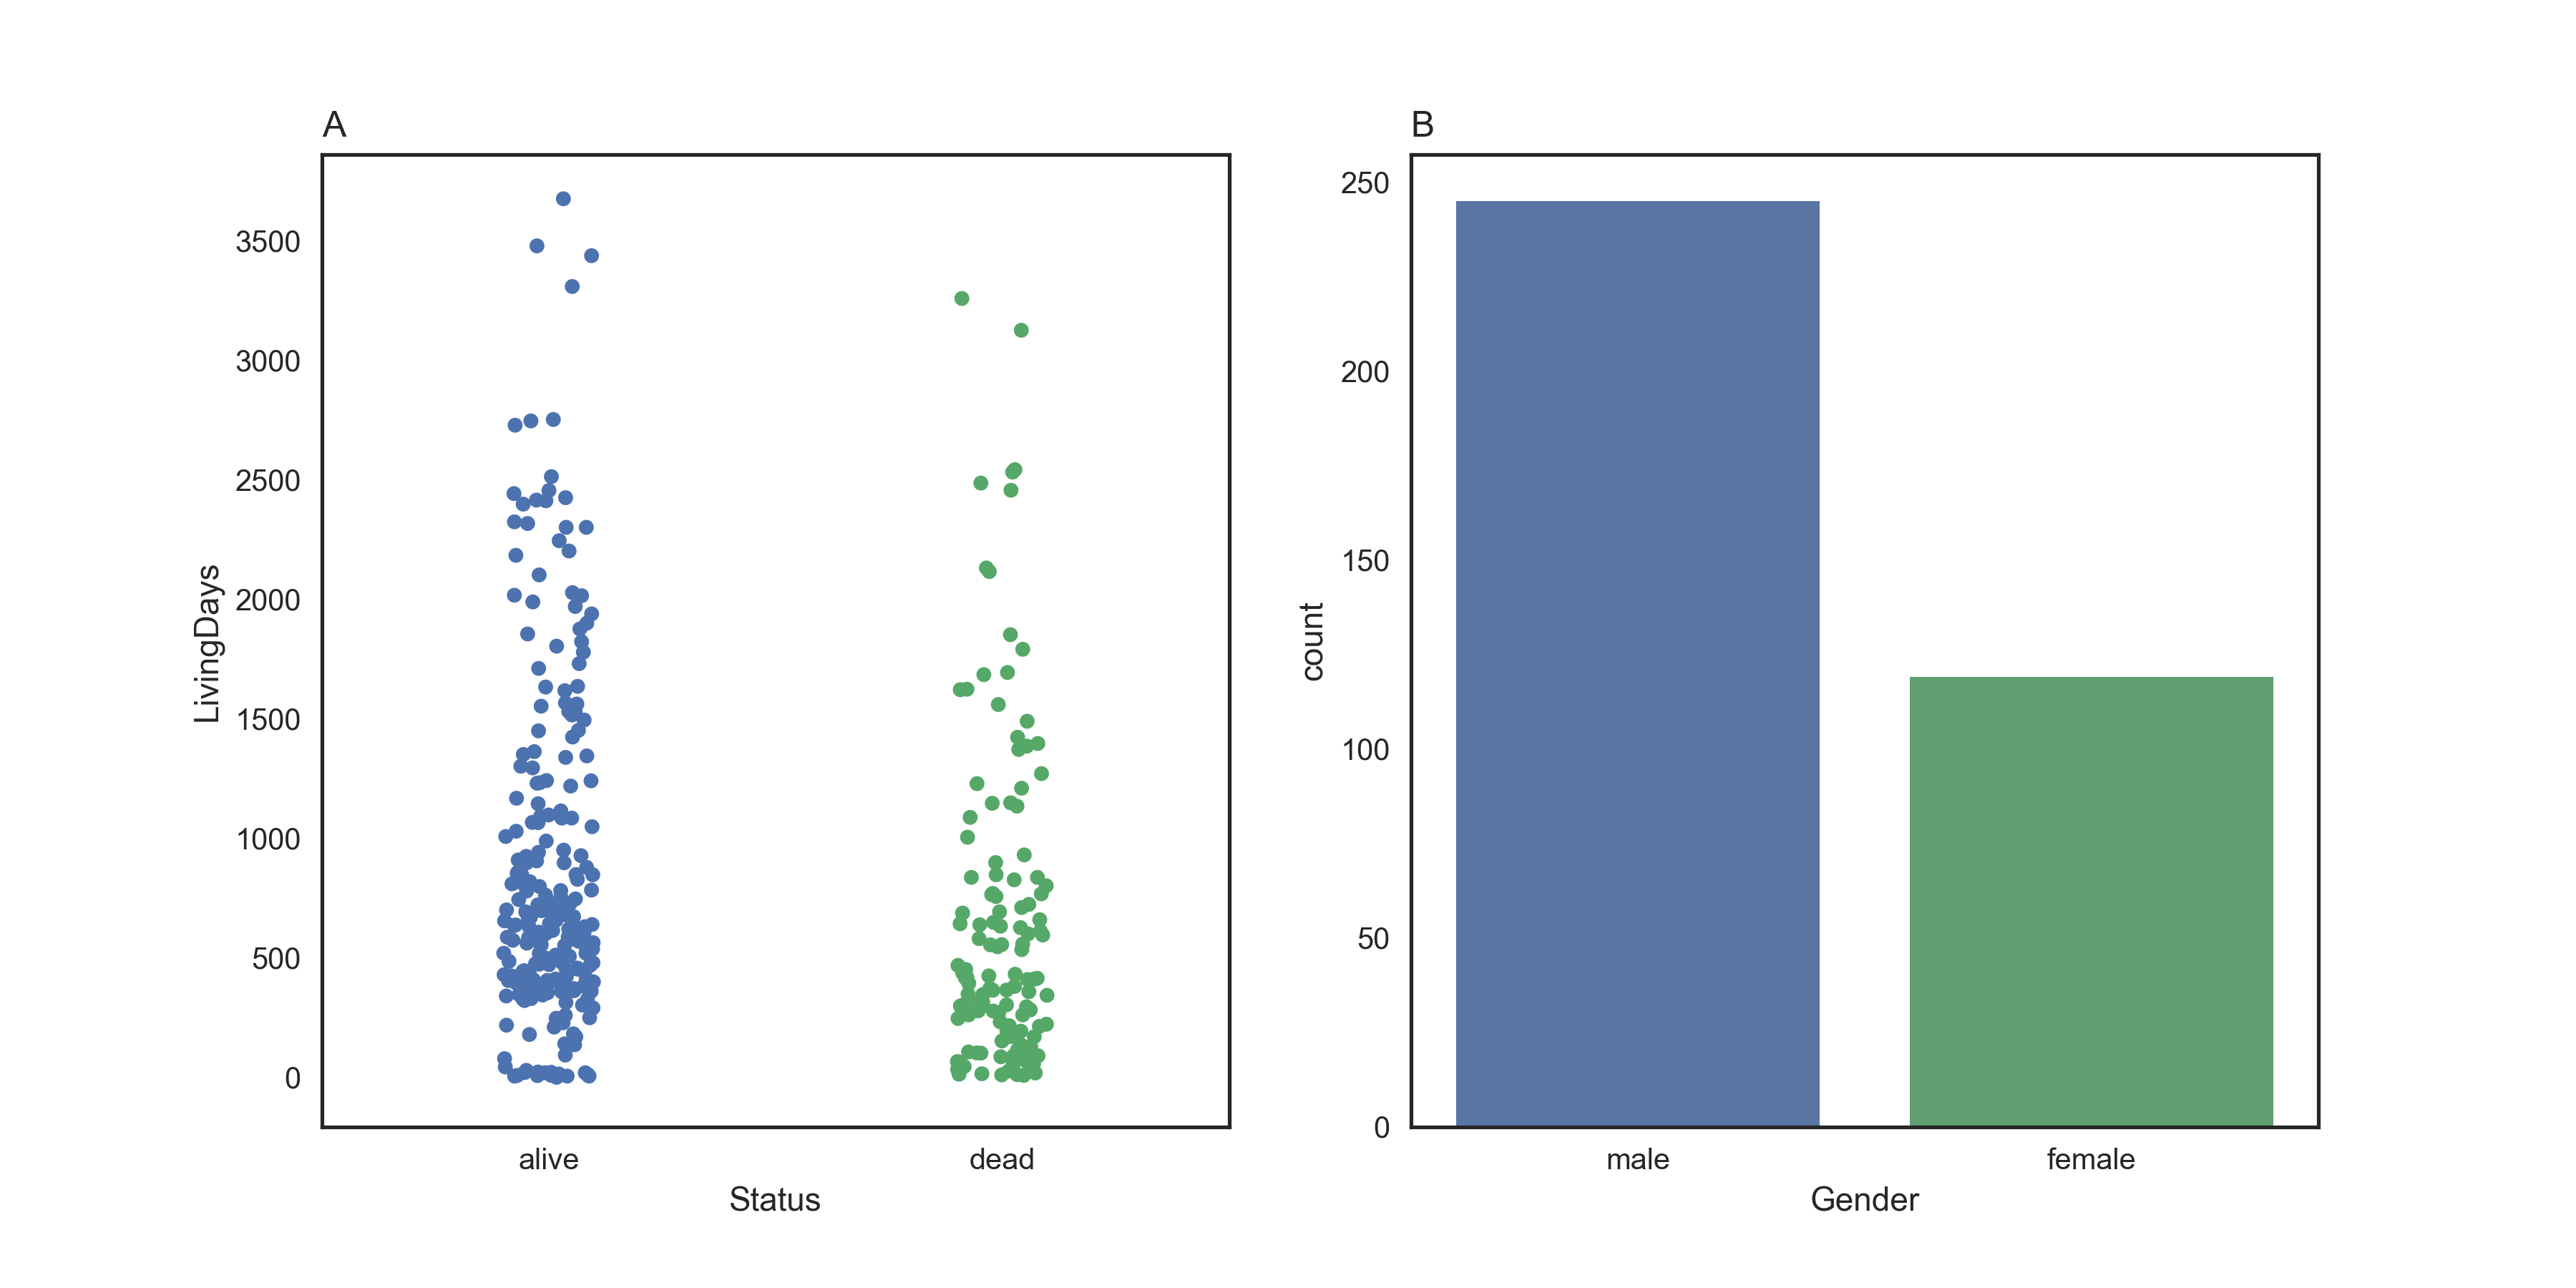
\includegraphics[width=0.75\textwidth]{Genderandstatus.png}
    \caption{A) Number of alive and dead patients in the liver cancer cohort, the number of alive patients are nearly twice as many as dead patients. B) Distribution of living days in two status group , alive and dead.\tiny}
    \label{fig:status_livingdays}
\end{figure}

	\subsection {Gene expression survival analysis with Cox regression model }
	
	The survival analysis requires the time period for the event to occur (in our case death). Thus , in liver cancer cohort variable living days was taken as time variable with status as hazard event. However, other variables had $NA$ available  some categorical features so these were not taken into consideration while building Cox regression hazard model implementation in lifeline module in python. Each transcript was taken as dependent variables in the model which gave us survival probabilities and cumulative hazard estimates for each transcript as shown in the figure~\ref{fig:Baseline_hazard_and_survival}. However not all the gene transcript ran into the model as these gene expression were spares and had missing expression data. These 130 features were excluded from the current analysis.  The cox regression model was run in 19219 gene transcripts completely which gave us hazard, survival function. These estimates provided the p-values as the measure of the significance of gene expression as prognostic marker for  liver cancer survival. Out of 19219 gene expression $6032$ gene expression was considered significant at p-value $< 0.05$. However these are raw p-value without taking into account Cox regression model was run for 19219 features.   
	
\begin{figure}[tbh]
    \centering
      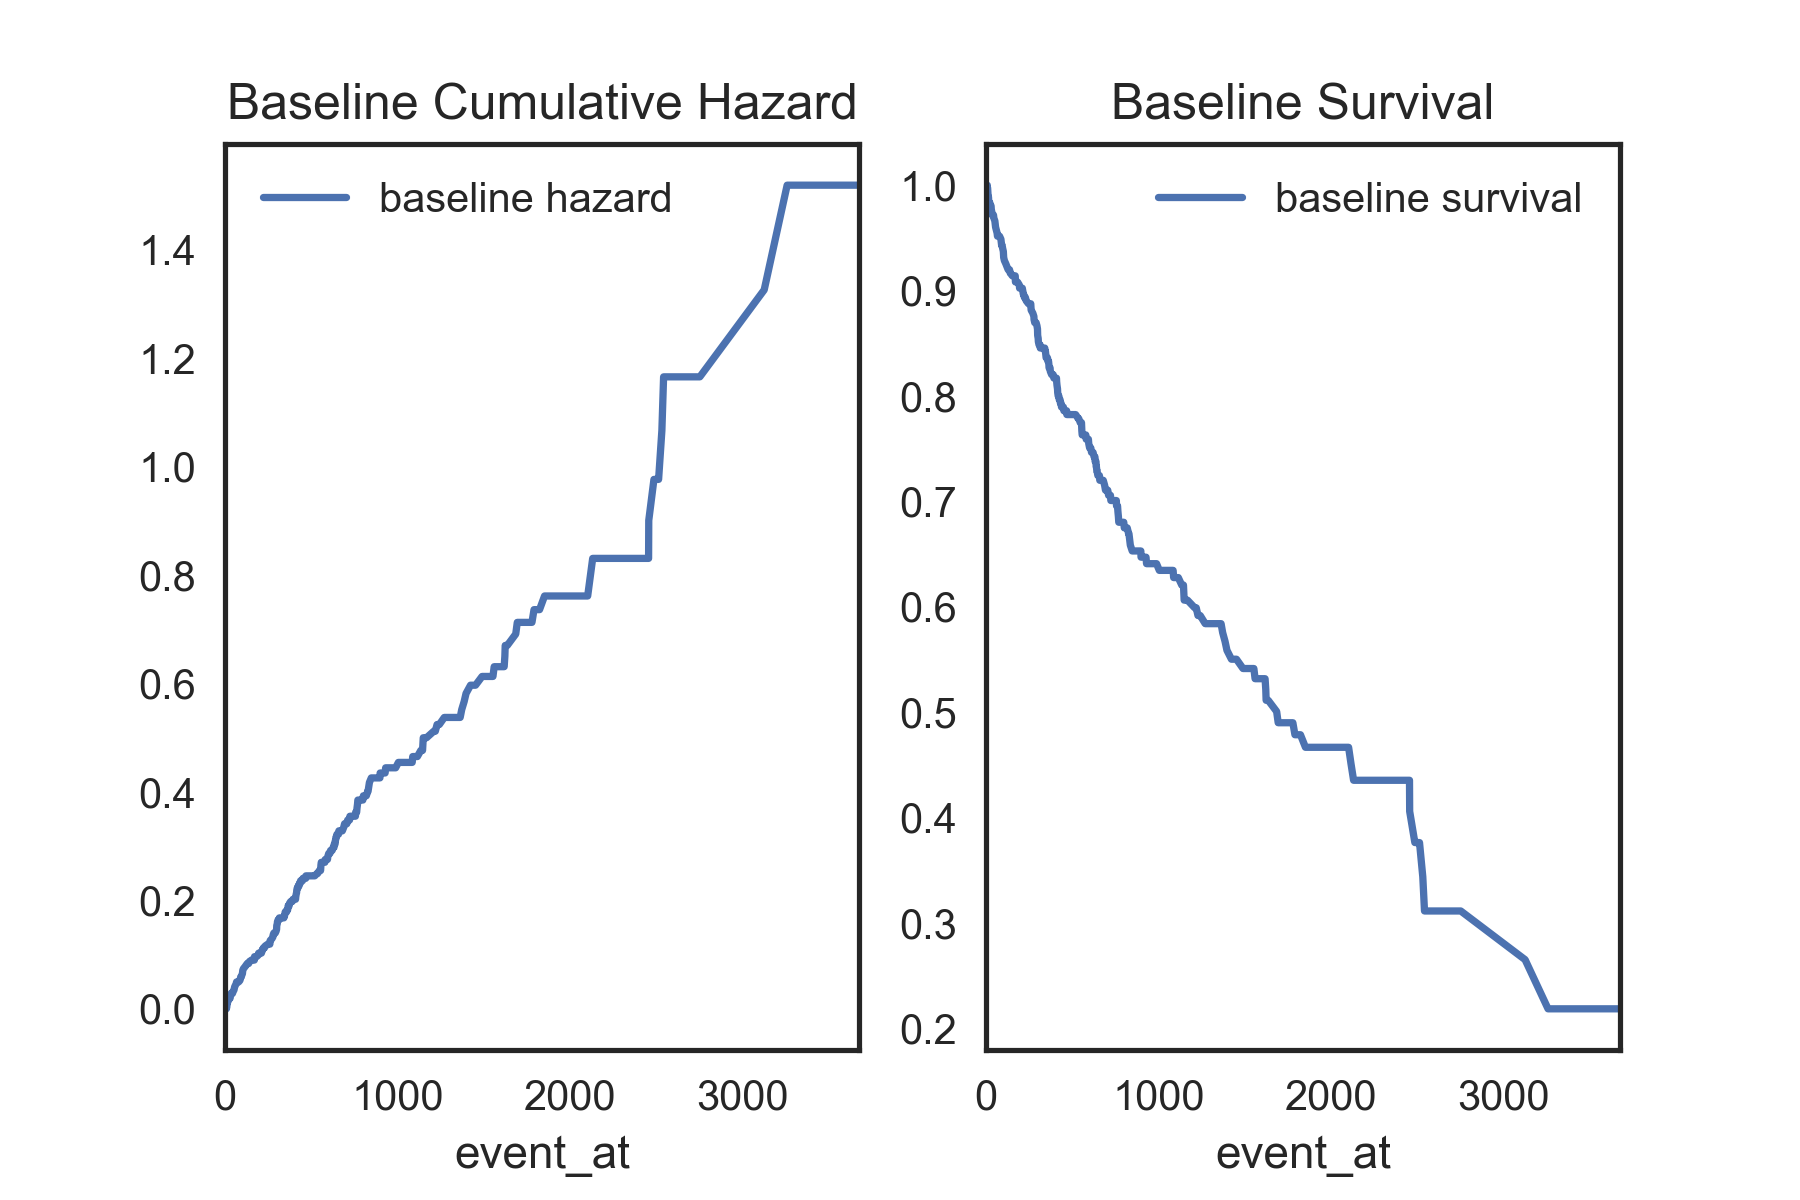
\includegraphics[width=0.75\textwidth]{survial_plot_one_mock_gene.png}
    \caption{The baseline cumulative hazard function for a mock gene transcript $ENSG00000000003$   The p-value for the transcript was $0.43$ with hazard coefficient of $-0.0057$ indicating that it is not a reliable prognostic marker of liver caner prognosis.}
    \label{fig:Baseline_hazard_and_survival}
\end{figure}
  		
	\subsection { Multiple hypothesis correction }
	
	\subsubsection {Estimating $\pi_0$ estimates on pvalues}
	
	Storey and Tibshirani \cite{storey2003statistical} provided the mathematical implementation for false positive discovery rate.  Using the implementation as discussed in the paper we calculated the $\pi_0$ estimates. Using the cublc spline fitting $\pi_0$ and  $\lambda$ values we calculated the  $\hat {\pi_0}$ for the p-values obtained from Cox model for each transcript as shown in figure~\ref{fig:estimate_pi}. The  $\hat {\pi_0}$  was estimated at $0.56$. 
\vspace{50cm} 
\begin{figure}
    \centering
     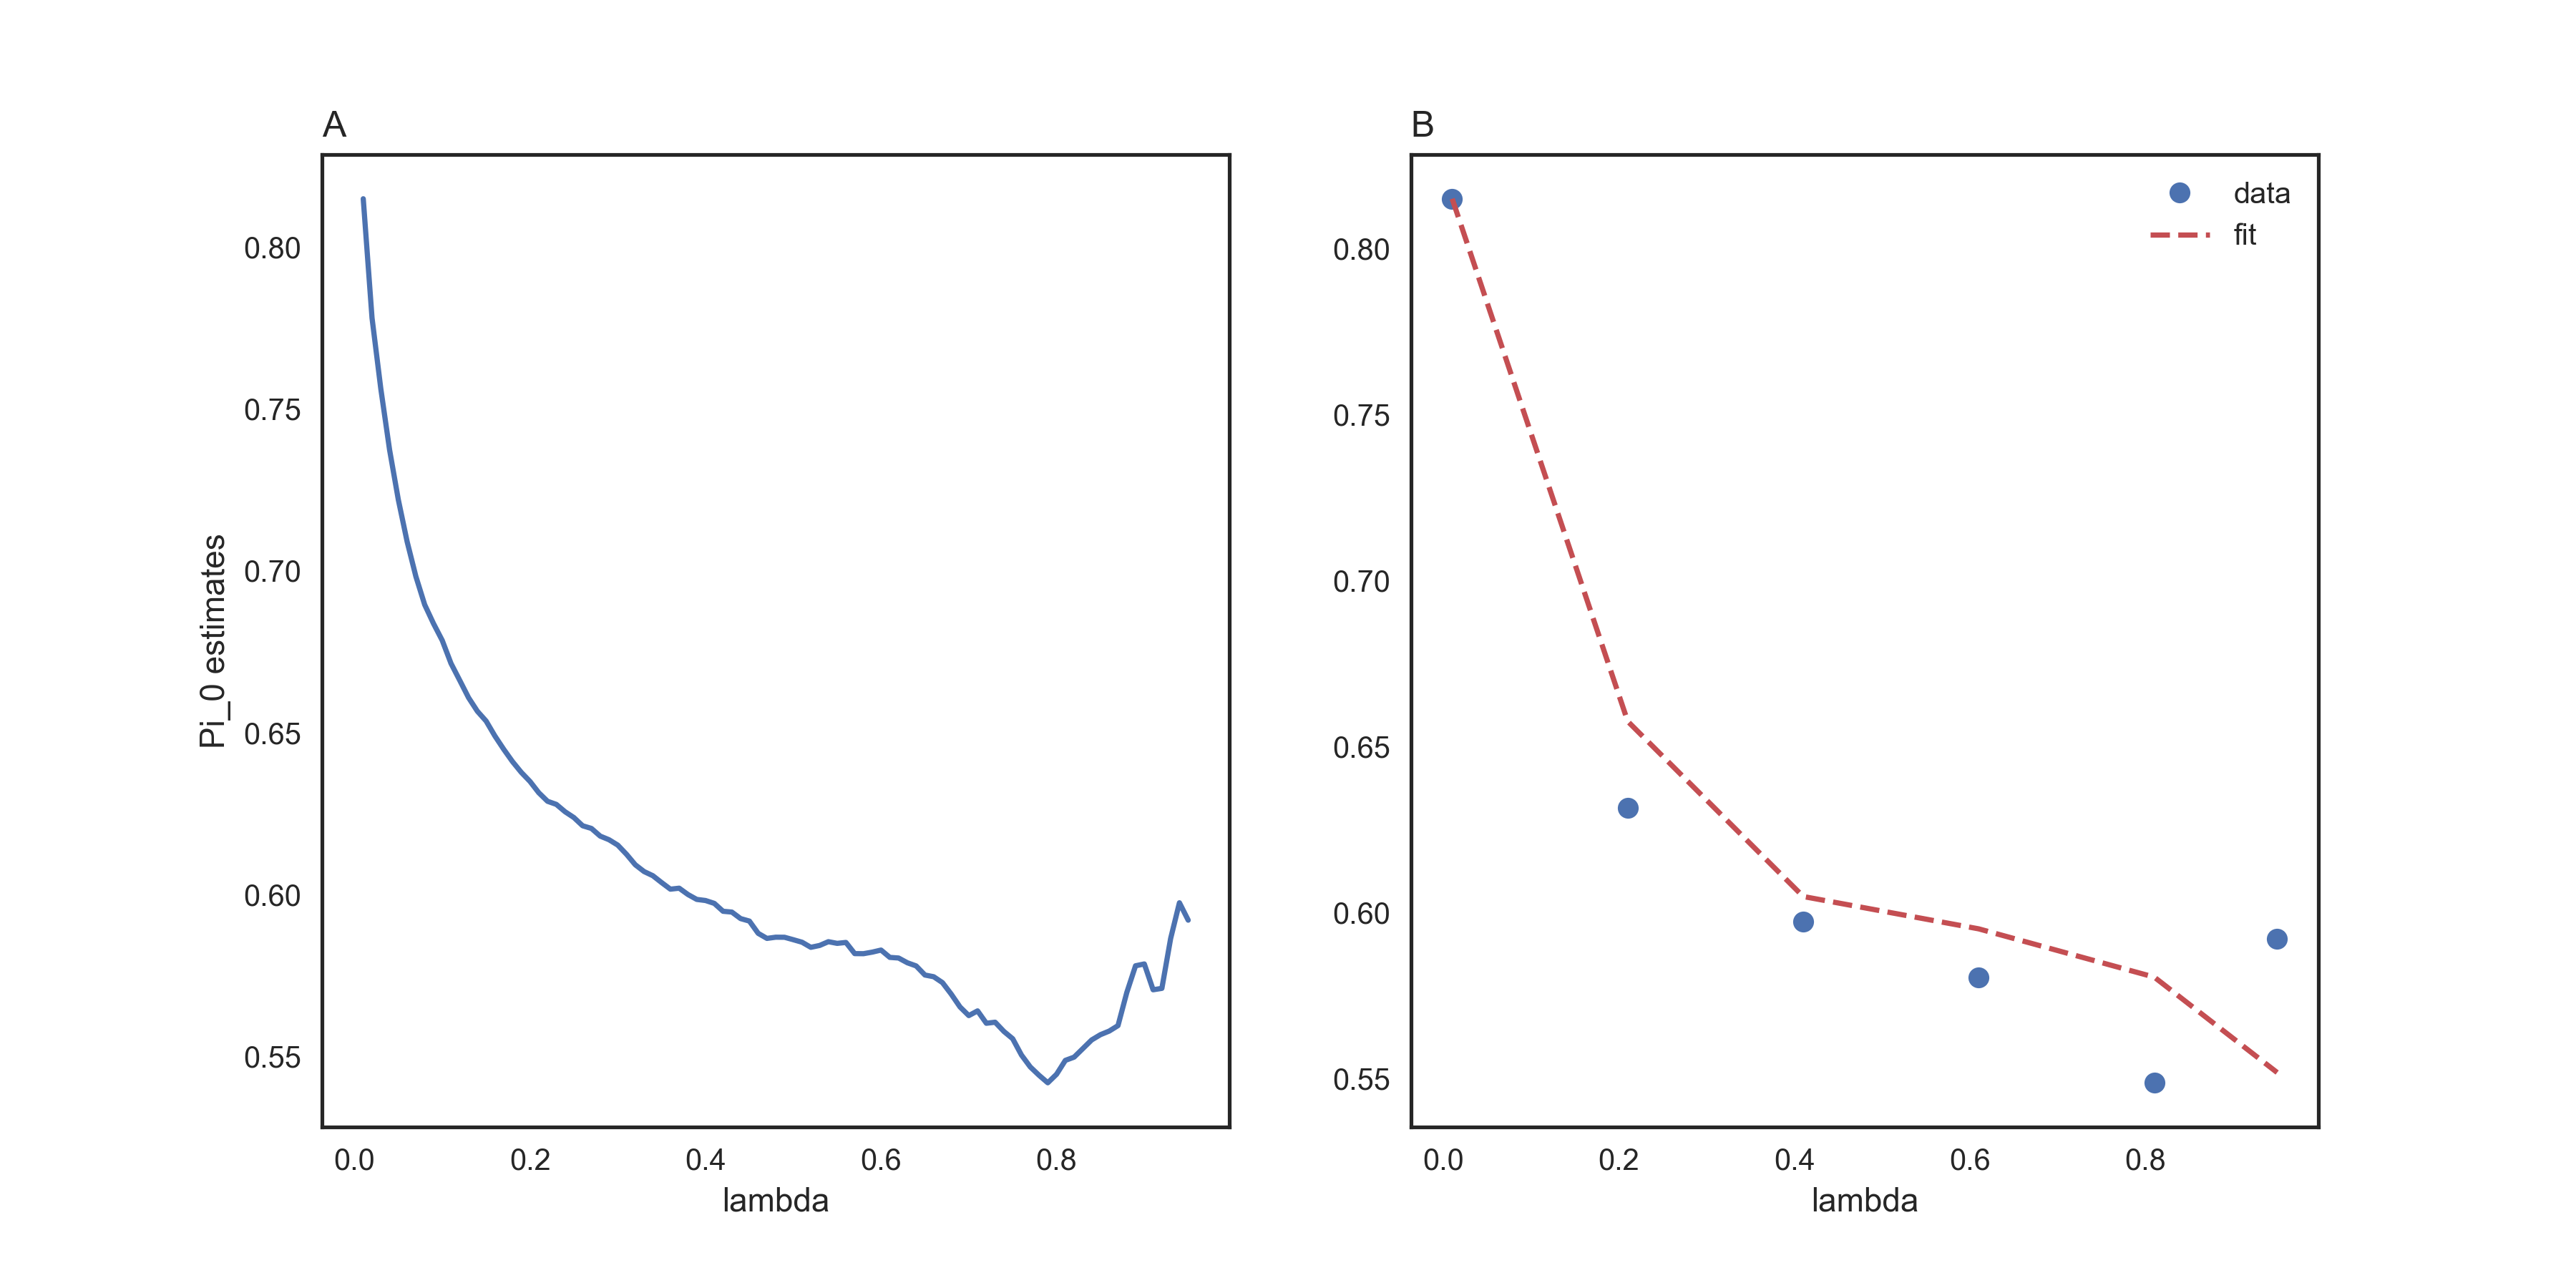
\includegraphics[width=\textwidth]{lambdaestimatescurvefitting.png}
    \caption{ A) $\pi_0$ estimates of $\lambda$  for $0.01$ to $0.95$ using the Storey and Tibshirani \cite{storey2003statistical} implementation in python. B) Cubic spline fitting to $\pi_0$  and $\lambda$ estimates. The blue points are subsets of real data and dotted lines are corresponding  fitted cublic spline   \tiny}
    \label{fig:estimate_pi}
\end{figure}

	\subsubsection {Estimation of q-values based on $\hat {\pi_0}$  values }
	 For each p-values of the transcript gene expression, a $\hat {\pi_0}$ $p_i$  was implemented in python in order to find the estimated q values for the  $i$th significant features using the equation as defined in Storey and Tibshirani \cite{storey2003statistical}. As shown in figure~\ref{fig:estimate_pi} we are able to control the false postive rates for p values calculated. We are able to find at least 4649 expressed gene transcript at $q$ $<$ $0.05$ . However considering the number of features tested we can further go to stricter cutoff such as $q < 0.01$ which would yield us 2464 gene transcript expression  as prognostic marker of liver cancer survival. 

	
\begin{figure}
\centering
     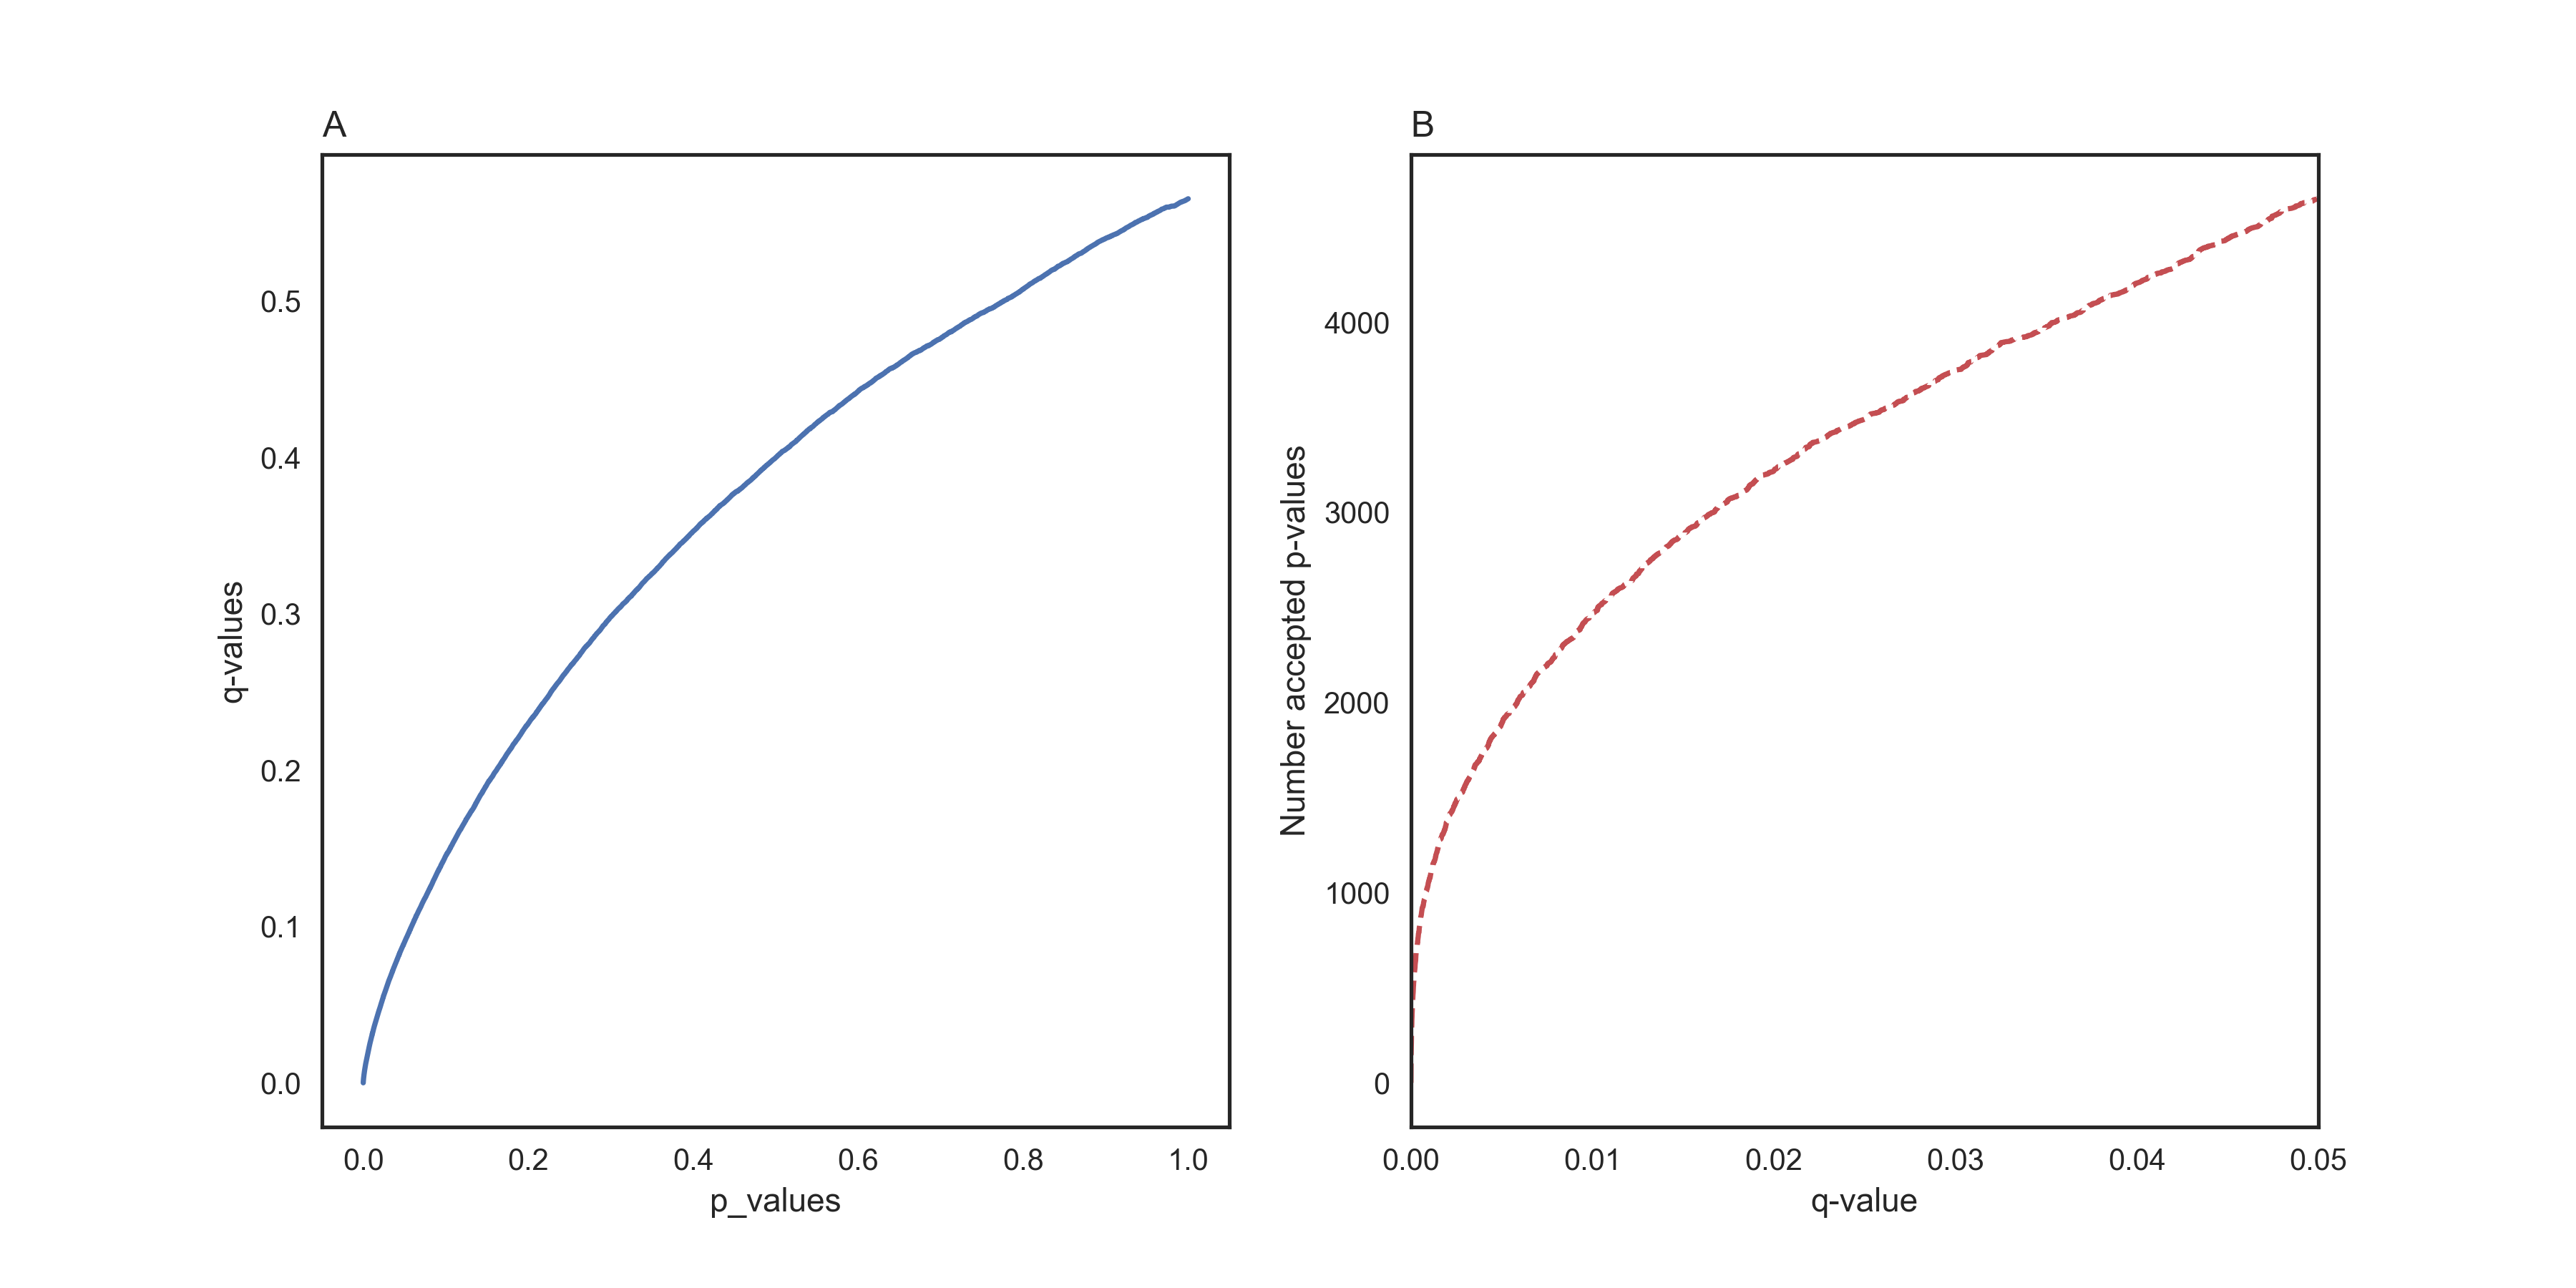
\includegraphics[width=1.1\textwidth]{comb.png}
    \caption{A) p VS q values for  different gene expression features. B) The number of $p$ values accepted at $q$ values $0.05$ . C) The number of $p$ values accepted at $q$ values $0.01$}
    \label{fig:animals}
\end{figure}



\newpage
\bibliographystyle{plain}
\bibliography{new_lib}

\end{document}